\subsection{可测函数的初等性质}

定理 1. --- 设 X 是一个局部紧空间，\(\mu\) 是 X 上的一个测度，\((\mathrm{F}_n)\) 是拓扑空间的一个序列，\(\mathbf{F} = \prod_{n} \mathbf{F}_n\) 是它们的乘积。对每个指标 \(n\)，设 \(f_n\) 是 X 到 \(\mathbf{F}_n\) 中的可测映射，并设 \(f(x) = (f_n(x)) \in \mathbf{F}\)；那么，对每个连续映射 \(u\)（\(f(\mathbf{X})\) 到拓扑空间 G 中的），函数 \(x \mapsto u(f(x))\) 都是可测的。

对 X 的每个紧子集 K 和每个数 \(\varepsilon > 0\)，存在紧集 \(K_{1} \subset K\)，使得 \(|\mu|(\mathrm{K} - \mathrm{K}_{1}) \leqslant \varepsilon\)，且在 \(K_{1}\) 上所有函数 \(f_{n}\) 的限制都是连续的（No.~1, 命题 2）；显然 \(u \circ f\) 在 \(K_{1}\) 上连续，由此即得定理。

注. --- 1) 该定理不能推广到拓扑空间的任意乘积（习题 1）。

\pandocbounded{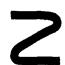
\includegraphics[keepaspectratio]{images/part001_9d1170b3.jpg}}

\begin{enumerate}
\def\labelenumi{\arabic{enumi})}
\setcounter{enumi}{1}
\tightlist
\item
  若 \(f\) 是 \(X\) 到其自身中的连续映射，而 \(g\) 是 \(X\) 到 \(F\) 中的可测映射，则 \(g \circ f\) 未必可测（习题 2）。
\end{enumerate}

推论 1. --- 有限多个可测数值函数（有限或非有限）的上包络与下包络都是可测的。

因为 \(\sup (u,v)\) 与 \(\inf (u,v)\) 在 \(\overline{\mathbf{R}}\times \overline{\mathbf{R}}\) 上连续

推论 2. --- 要使数值函数 \(f\)（有限或非有限）可测，必须且只需 \(f^{+}\) 与 \(f^{-}\) 可测。

条件是必要的，由推论 1 即得；它是充分的，因为 X 在 \(\overline{R} \times \overline{R}\) 中的像 A（在映射 \(x \mapsto (f^{+}(x), f^{-}(x))\) 下）不含点 \((+\infty, +\infty)\) 与 \((-\infty, -\infty)\)，从而映射 \((u, v) \mapsto u - v\) 在 A 上连续。

推论 3. --- 若 f 与 g 是 X 到拓扑向量空间 F 中的两个可测映射，则 \(f + g\) 与 \(\alpha f\) 都是可测的（ \(\alpha\) 为任意标量）。

因此，X 到拓扑向量空间 F 中的可测映射所成之集是一个向量空间。

推论 4. --- 设 F 是 R 上的一个 n 维向量空间，并设 \((\mathbf{e}_{k})_{1\leqslant k\leqslant n}\) 是 F 的一个基。要使函数 \(f=\sum_{k=1}^{n}\mathbf{e}_{k}f_{k}\) 可测，必须且只需每个数值函数 \(f_{k}\) 都可测。

推论 5. --- 设 F、G、H 是三个拓扑向量空间，并设 \((u, v) \to [u \cdot v]\) 是 \(F \times G\) 到 H 中的一个连续双线性映射。若 f 是 X 到 F 中的可测映射，g 是 X 到 G 中的可测映射，则 \([f \cdot g]\) 是 X 到 H 中的可测映射。

特别地，若 f 是 X 到实（相应地，复）赋范空间 F 中的可测映射，而 g 是 X 到 R（相应地，C）中的可测映射，则 gf 可测。若 F 是一个赋范代数，且 f、g 是 X 到 F 中的两个可测映射，则 fg 可测。

推论 6. --- 若 f 是 X 到赋范空间 F 中的可测映射，则数值函数 \(|f|\) 是可测的。

